\documentclass[fleqn,varvw,preprintnumbers,citeautoscript]{memo}

\usepackage[utf8]{inputenc}
\usepackage[T1]{fontenc}

\graphicspath{{../../fig/}}
\usepackage[caption=false]{subfig}
\usepackage{enumerate}
\usepackage{listings}


\newcommand\vlong{V_\text{long}}

\begin{document}

\title{Memo 3: schema circuitale completo}

\author{Francesco Polleri}
\email{s5025011@studenti.unige.it}
\author{Mattia Sotgia}
\email{s4942225@studenti.unige.it}

\collaboration{Gruppo A1}
\affiliation{Dipartimento di Fisica, Università degli Studi di Genova, I-16146 Genova, Italia}

\author{Lorenzo Lucentini}
\author{Michele Giorgi}
\collaboration{Gruppo C6}
\affiliation{Dipartimento di Fisica, Università degli Studi di Genova, I-16146 Genova, Italia}

\revised{\today}
\preprint{MEMO/3 (\today)}

\begin{abstract}

\end{abstract}
\maketitle

\section{I/O sistema di controllo}

\begin{enumerate}
    \item \verb-A0 (INPUT)-: lettura della tensione in uscita dall'amplificatore operazionale per strumentazione;
    \item \verb-A1 (OUTPUT)-: scrittura del valore di riferimento $V_\times$ per il comparatore (deve essere compreso tra 0 V e il valore massimo assumibile (\SI{5}{\volt} (MEGA 2560) o \SI{3.3}{\volt} (DUE));
    \item \verb-A3 (INPUT)-: lettura della tensione in entrata al generatore/sonda (valore atteso di $+$\SI{5}{\volt} (MEGA 2560) o $+$\SI{3.3}{\volt} (DUE));
    \item \verb-D2 (GPIO/OUTPUT)-: Scrittura per avere $+$\SI{5}{\volt} (MEGA 2560) o $+$\SI{3.3}{\volt} (DUE) in uscita per alimentare il generatore di corrente.
    \item \verb-GND- collegato a terra;
    \item \verb-D14/D14_TX3 (OUTPUT/SERIAL3)-: utilizzato per la comunicazione seriale con il generatore PL303QMD-P, in ingresso al comparatore sull'input invertente. 
\end{enumerate}

\section{Logica di controllo e misura}

\begin{enumerate}
    \item chiamata a \verb-init()-;
    \item \verb-Serial.begin(9600)- e \verb-Serial3.begin(9600)-
    \item Setup \verb-I/O- pins: 
    \begin{enumerate}
        \item \verb-A0-: output,
        \item \verb-A1-: input,
        \item \verb-D2-: output;
        \item \verb-A3-: input;
    \end{enumerate}
    \item Imposto il valore di \verb-A1- al riferimento $V_\times$ (circa \SI{2.5}{\volt}?)
    \item Impostare i limiti di $V_\text{max}$ per il generatore/elettromagnete sul seriale (comando \verb-'V1 30'-);
    \item Imposto limite corrente a zero \verb-'I1 0'-;
    \item Accendo il canale 1 del generatore/elettromagnete \verb-'OP1 1'-.
    \item Attendo un segnale di start della misura dal seriale con il computer (\verb+REMOTE:START?+), invio una conferma di ricezione (\verb+INO:RUN+) e il computer inizia a raccogliere quindi le misure che sono inviate sul seriale.
    \item Loop sulle $M$ correnti (da \SI{0}{\ampere} a \SI{1.2}{\ampere} in incrementi da \SI{0.1}{\ampere}): \begin{enumerate}
        \item Imposto la corrente al valore successivo (incrementi da \SI{0.1}{\ampere});
        \item Loop su un contatore da 0 a $N=100$, incrementi di 1: \begin{enumerate}
            \item Attivo la corrente che va alla sonda (imposto il pin \verb-D2- su \verb-HIGH-);
            \item Eseguo misura di $V_\text{op-amp}$ (pin \verb-A0-) e di $V_\text{gen}$ (pin \verb-A3-), scrivo i file sul seriale (e in un array di dimensione $12\times100$, all'indice $i$ su cui sto iterando rispetto a $M$ e $j$ rispetto a $N$);
            \item Disattivo la corrente che va alla sonda (imposto il pin \verb-D2- su \verb-HIGH-);
            \item Eseguo misura di $V_\text{op-amp}^\text{off}$ (pin \verb-A0-) e di $V_\text{gen}^\text{off}$ (pin \verb-A3-), scrivo i file sul seriale (e in un array di dimensione $12\times100$, all'indice $i$ su cui sto iterando rispetto a $M$ e $j$ rispetto a $N$);
        \end{enumerate}
    \end{enumerate}
    \item Spengo il generatore, impostando \verb-'V1 0'-, 1verb-'I1 0'- e poi \verb-'OP1 0'-;
    \item Segnale \verb-INO:STOP- sul seriale con il computer, fine delle misure;
\end{enumerate}

\subsection{logica del programma di lettura del seriale}

Il programma di lettura del seriale scritto in python è equivalente ad un mirror perfetto del programma scritto per la scheda di ocntrollo, in quanto deve leggere i dati da seriale, salvarli e poi calcolare i valori medi, che anche salverà su un file \verb-.root-. Il programma consente anche di controllare in remoto l'acquisizione da parte della scheda utilizzando una comunicazione seriale. 

%\begin{lstlisting}[morekeywords={init},columns=flexible]
%init();
%(Serial && Serial3).begin(9600)
%
%\end{lstlisting}


\begin{turnpage}
    \begin{figure*}[p]
        \centering
        % 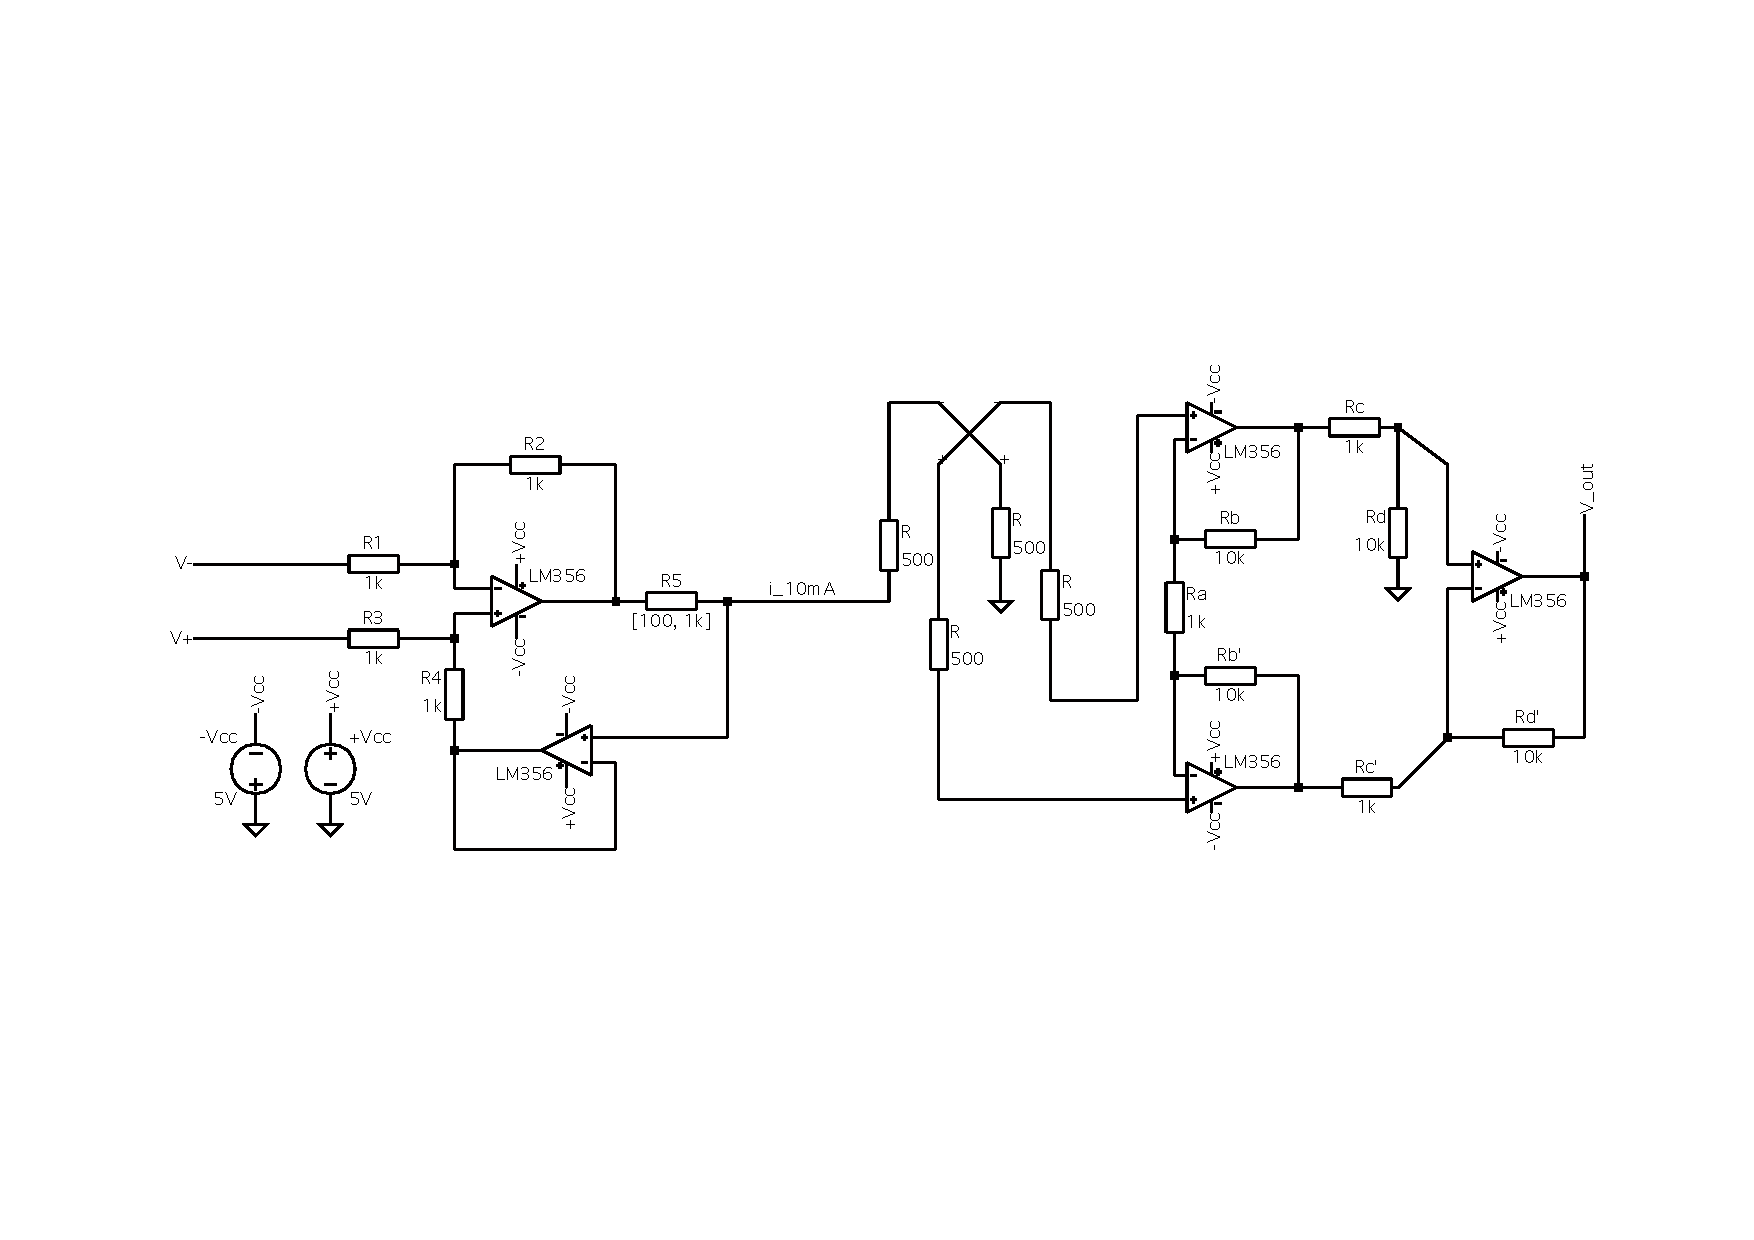
\includegraphics[width=\linewidth,trim={2cm 6.5cm 2cm 6cm},clip]{memo2_full_circuit.pdf}
        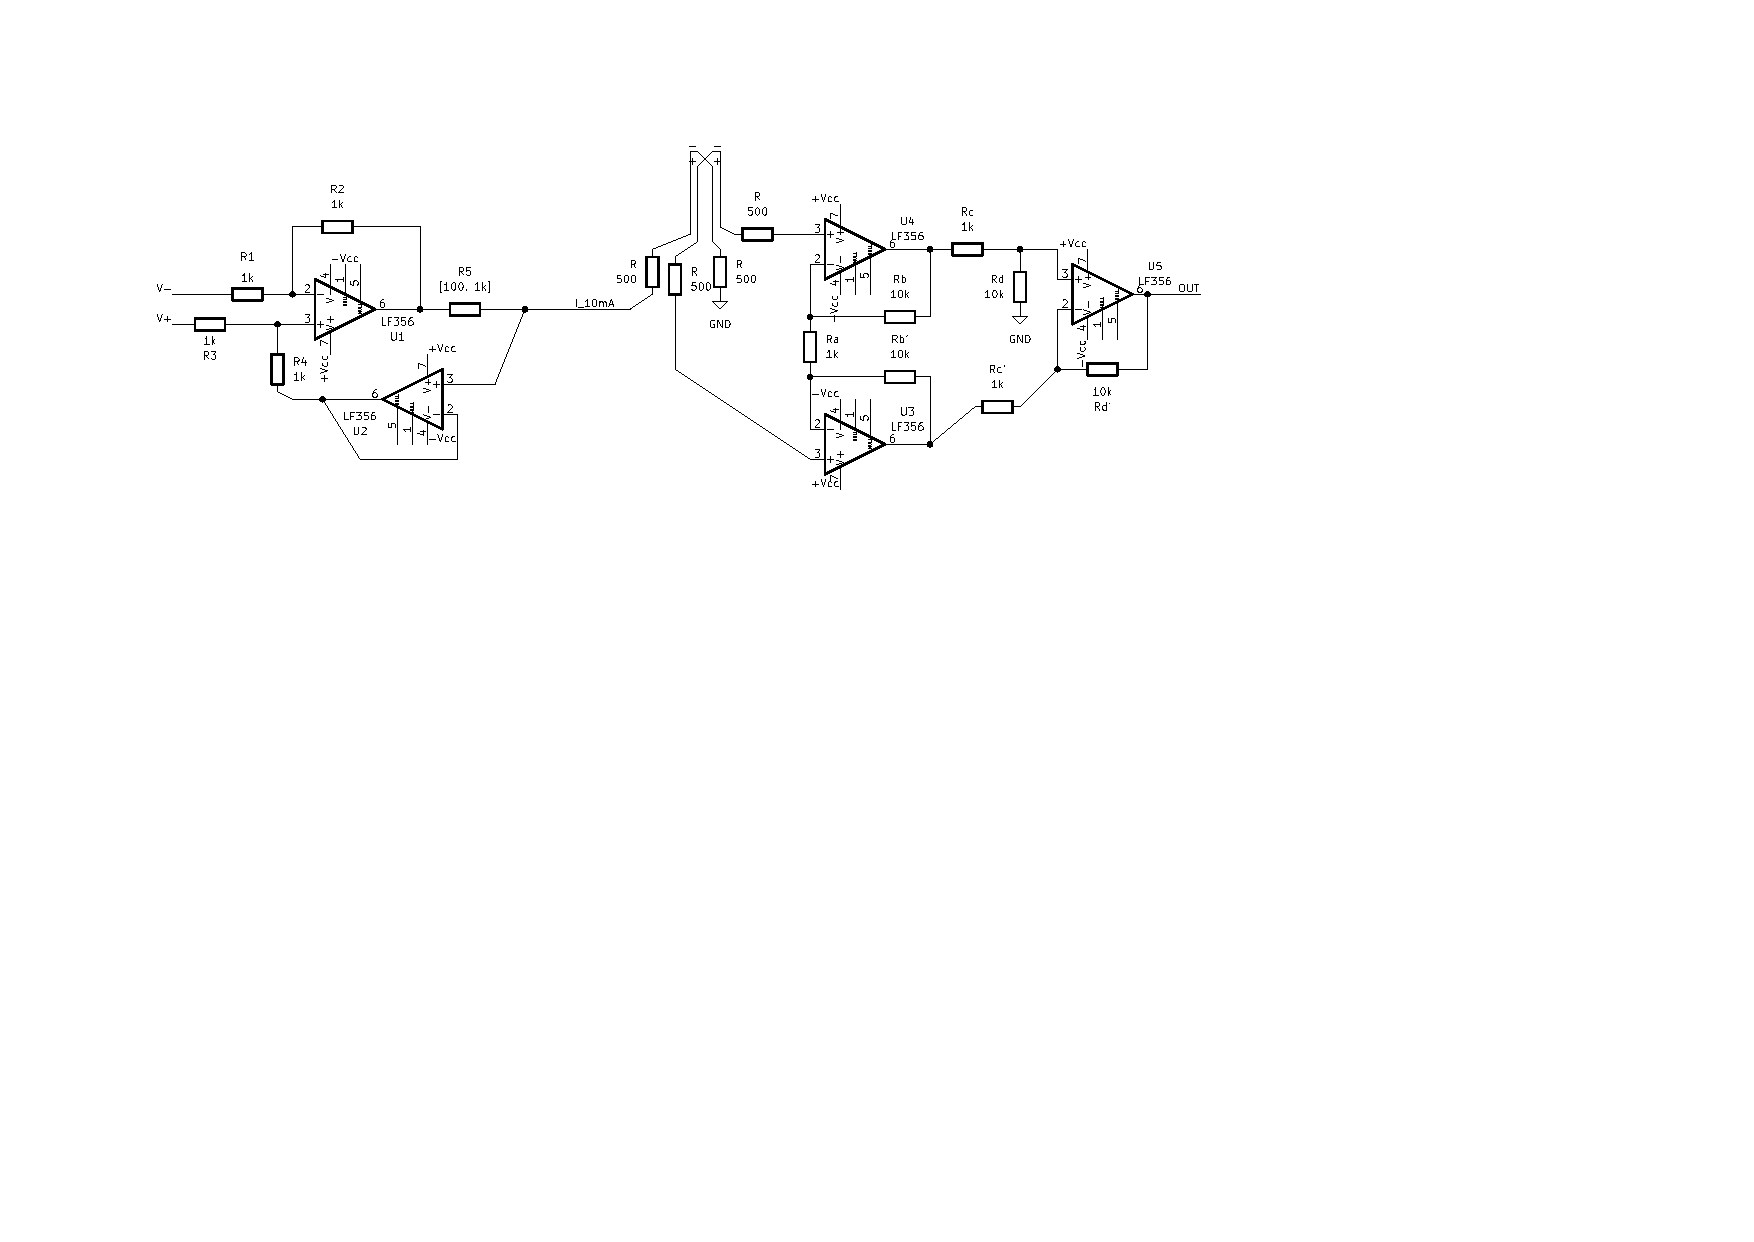
\includegraphics[width=\linewidth,trim={1.5cm 3.5cm 2cm 2cm},clip]{SCHEMA_full1.pdf}
        \caption{Circuito completo delle tre componenti principali (da sinistra a destra sono inseriti il generatore di corrente, la sonda e l'amplificatore differenziale per strumentazione). In basso a destra troviamo la scheda Arduino MEGA 2560 mappata sui pin utilizzati per il setup sperimentale. }\label{fig:circuit_memo2}
    \end{figure*}
\end{turnpage}

\end{document}